\chapter{Generalized Covariance Union}\label{chapter:gcu}

\section{Data Fusion Framework}\label{section:framework}

\PARstart{C}{ovariance Union}, in both its Optimal and Generalized forms, is part of a larger hierarchy of data fusion
tools which when used properly together cover a broad range of possible situations, and form a robust framework with
which to build higher-level applications~\cite{fusion06,uhlmann03}. The remainder of this section is given to present
the previously published portions of this framework, the Kalman filter, Covariance Intersection, and Optimal Covariance
Union; both as background information and to provide the proper context for Generalized Covariance Union, which is 
detailed in sections \ref{section:motivation} and \ref{section:gcu}.


% SECTION Kalman
\subsection{Kalman Filter}

The most basic concept of data fusion is the idea that two pieces of information can be ``fused'' to create
a new piece of information which is ``better'' than the two inputs by some metric. One tool used to perform this action
is the Kalman filter. The Kalman filter addresses the general problem of trying to estimate the state $\v{x}\in\Re$  of
a discrete-time controlled process that is governed by the linear stochastic difference equation
\begin{equation}\label{eqn:kalsto}
    \v{x}_k = \m{A}\v{x}_{k-1} + \m{B}\v{u}_k + \v{w}_{k-1} ,
\end{equation}
with a measurement $\v{z}\in\Re$ that is
\begin{equation}\label{eqn:kalmeasure}
\v{z}_k = \m{H}\v{x}_k + \v{v}_k.
\end{equation}
where $\v{w}_k$ and $\v{v}_k$ are random variables which represent the process and measurement noise, respectively,
where $\m{H}_i$ is the transformation for the state space of the fused estimate to the state space of the
estimate~\cite{siggraph01}.

The filter operates in two steps for every discrete unit of time. The first step is the projection step, in which the 
future state of a system is estimated, projecting forward from time step $k-1$ to the current time step $k$. This is 
given by
\begin{align}
    \v{x}^-_k &= \m{A}\v{x}_{k-1}+\m{B}\v{u}_k\\
    \m{P}^-_k &= \m{A}\m{P}_{k-1}\m{A}^T+\m{Q}
\end{align}
where $\m{Q}$ is the process noise covariance defining the PDF for the variable $\v{w}_k$ from equation \ref{eqn:kalsto}.
The second step is the update step, in which the actual measurements are used to correct the predicted state. This is
given by
\begin{align}
    \v{x}_k &= \v{x}^-_k+\m{K}_k(\v{z}_k-\m{H}\v{x}^-_k)\\
    \m{P}_k &= (\m{I}-\m{K}_k\m{H})\m{P}^-_k,\\
\intertext{with}
    \m{K}_k &= \m{P}^-_k\m{H}^T(\m{H}\m{P}^-_k\m{H}^T+\m{R})^{-1},
\end{align}
where $\m{R}$ is the measurement noise covariance defining the PDF for the variable $\v{v}_k$ from equation
\ref{eqn:kalmeasure}~\cite{siggraph01}.

In addition to a time-sequence of measurements received from the same source, the Kalman filter may also be applied to a
set of separate measurements from different sources. Given a set of statistically {\em independent} (uncorrelated) estimates
$(\v{m}_1,\m{M}_1),(\v{m}_2,\m{M}_2),\dots,(\v{m}_n,\m{M}_n)$, the Kalman fusion equations can be written
as~\cite{uhlmann03,maybeck79}
\begin{figure}[tbp]
    \centering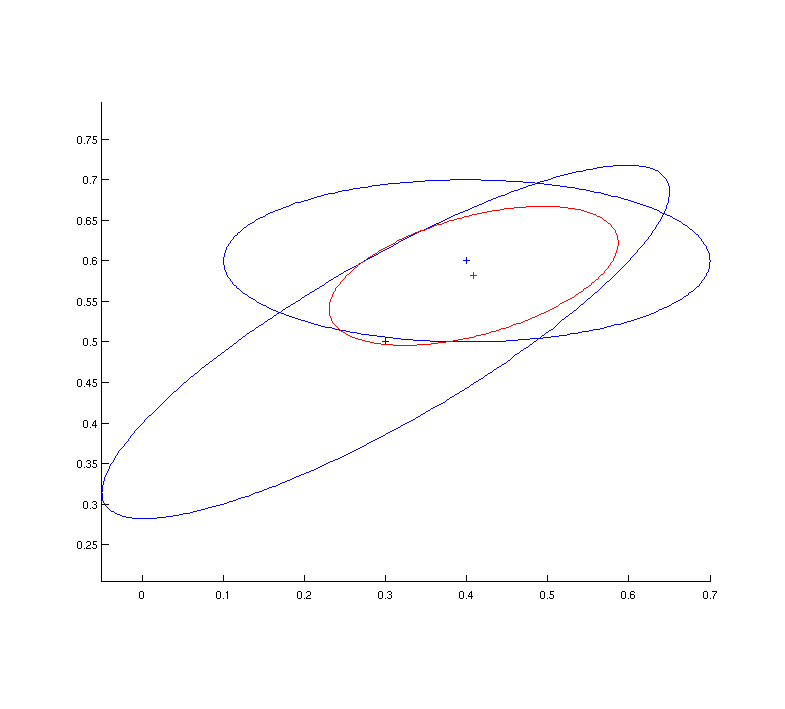
\includegraphics[width=0.6\textwidth]{figures/kalman2d.png}
    \caption{\it 1-$\sigma$ contour plots of two 2D inputs (blue) together with the Kalman fused result (red). Note that
        these contours are a distance of $\sigma$ away from the mean on a 2D Gaussian surface, and do not represent a
        closed volume or area. }
    \label{fig:kalman2d}
\end{figure}
\begin{align}
    \m{C} &= (\m{M}^{-1}_1+\m{M}^{-1}_2+\dots+\m{M}^{-1}_n)^{-1}\label{eqn:kalmanP}\\
    \v{c} &= \m{C}(\m{M}^{-1}_1\v{m}_1+\m{M}^{-1}_2\v{m}_2+\dots+\m{M}^{-1}_n\v{m}_n).\label{eqn:kalmanx}
\end{align}
Figure \ref{fig:kalman2d} illustrates the correct operation of the Kalman filter on two estimates known to be both
consistent and independent. Although the two input estimates and the fused Kalman result in the example are all 2D
Gaussian surfaces (which are greater than or equal to some unknown underlying PDF), it is convenient to represent these
probabilistic models simply by showing the 1-$\sigma$ contour centered at the mean.

In either form, the underlying assumptions in all Kalman applications are consistency and independence. However, any
presumption of statistical independence should be carefully considered, since virtually any sensor is subject to
time-correlated errors resulting from the particular conditions of its use; additionally errors associated with the 
non-linear transformation of its measurements are deterministic and therefore non-independent~\cite{uhlmann03}. For
example, any changes in temperature, barometric pressure, or humidity which affect the operation of a sensor's internal
electronics, and their effect on the sensor's accuracy, must be known {\em exactly}, or the assumption of independence
does not hold.
\begin{figure}[tbp]
    \centering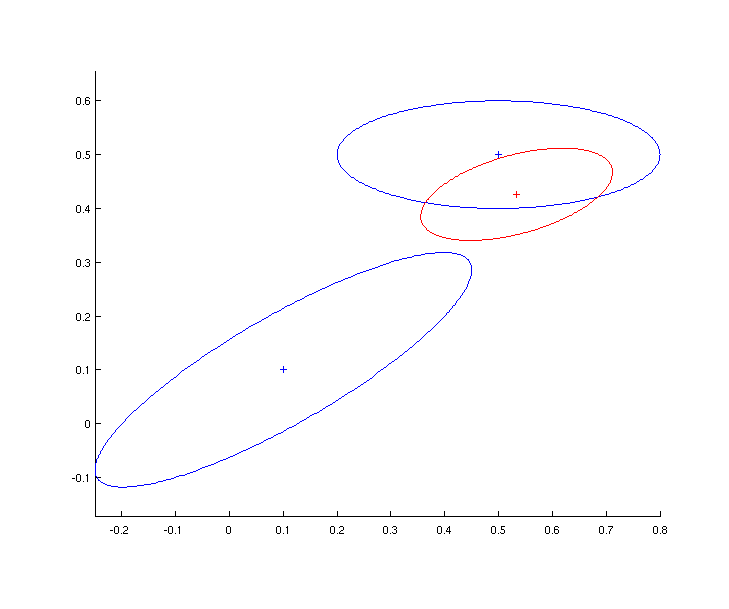
\includegraphics[width=0.6\textwidth]{figures/kalman2d-i.png}
    \caption{\it 1-$\sigma$ contour plots of two 2D inputs (blue) together with the Kalman fused result (red),
        illustrating a potentially inconsistent result. Note that the 1-$\sigma$ contours of the inputs, which are
        supposed to be independent estimates of the same position, do not overlap, suggesting that one may be the result
        of spurious data. One of the means is clear outlier when compared to the Kalman contour.}
    \label{fig:kalman2d-i}
\end{figure}
Figure \ref{fig:kalman2d-i} shows an example of what happens when the precondition for consistency is violated. The two
input estimates in this example are interpreted by the Kalman filter to be estimates of the same position, yet they are
far enough apart to suggest that one estimate might be the result of spurious data. Note that the 2D Gaussian surfaces
represented by the plotted 1-$\sigma$ contours do overlap, but not in the part of the surface that contains the highest
probability. The Kalman result shown will most likely not be consistent, but there is no way to correct for this
behavior.

To reiterate, the Kalman filter operates correctly if all its estimates are both consistent and independent.


% SECTION 1.2 CI
\subsection{Covariance Intersection}

Consider here the fusion of two estimates using either the Kalman filter or the data fusion technique known as
Covariance Intersection (CI), under the following circumstances:~\cite{uhlmann03}
\begin{enumerate}
\item {\em The two estimates are independent.} In this case the Kalman filter produces an optimal fused estimate while
CI produces a consistent, though suboptimal, estimate.
\item {\em The two estimates are completely correlated.} In this case CI produces an optimal fused estimate while
Kalman produces an inconsistent estimate.
\item {\em The two estimates are partially correlated.} In this case CI produces a consistent, though suboptimal,
estimate while the Kalman filter produces an inconsistent estimate.  \end{enumerate}
In each case, CI produces a consistent result, allowing it to operate safely in conditions which cause the Kalman filter
to fail.

The formulation of the CI equations follows from the joint covariance structure which exists between a given pair of
estimates $(\v{m}_1,\m{M}_1)$ and $(\v{m}_2,\m{M}_2)$
\begin{equation}\label{eqn:jointcov}
\left[\begin{array}{cc}
    \m{M}_1 & \m{X} \\
    \m{X}^T & \m{M}_2
\end{array}\right]
\end{equation}
where $\m{X}$ represents the actual, but unknown, cross covariance between the two estimates~\cite{uhlmann03}. Without
complete and exact knowledge of $\m{X}$, the only way to ensure consistency is to identify a joint covariance that is
guaranteed to be consistent based on the information available. This can be achieved by selecting a scalar value
$\omega, 0\leq1,$ and verifying that
\begin{equation}\label{eqn:cijointcov}
\left[\begin{array}{cc}
    \frac{1}{\omega}\m{M}_1 & 0 \\
    0                       & \frac{1}{1-\omega}\m{M}_2
\end{array}\right]
\leq
\left[\begin{array}{cc}
    \m{M}_1 & \m{X} \\
    \m{X}^T & \m{M}_2
\end{array}\right].
\end{equation}


This formulation of the $\omega$-parametrized covariance can be expanded from $2$ to $n$ estimates as follows
\begin{equation}\label{eqn:ncijointcov}
\left[\begin{array}{cccc}
    \omega_1\m{M}^{-1}_1 &                    0 &                    0 &                    0 \\
                       0 & \omega_2\m{M}^{-1}_2 &                    0 &                    0 \\
                       0 &                    0 &               \ddots &                    0 \\
                       0 &                    0 &                    0 & \omega_n\m{M}^{-1}_n
\end{array}\right],
\end{equation}
by selecting $\omega_1\dots\omega_n$ such that $1=\sum_{i=1}^n\omega_i$. By applying the inverse Kalman filter equations
\ref{eqn:kalmanP} and \ref{eqn:kalmanx} to \ref{eqn:ncijointcov}, the CI fusion equations for $n$ estimates with 
completely unknown degrees of correlation can be written as
\begin{figure}[tbp]
    \centering
        \subfloat[$\omega_1$=0.05]{\label{fig:ci2d05}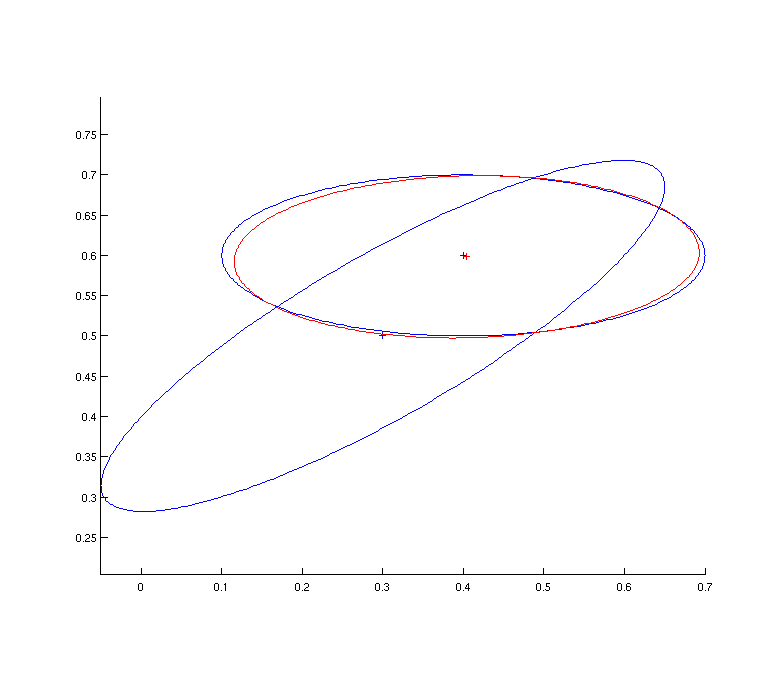
\includegraphics[width=0.4\textwidth]{figures/ci2d-05.png}}
        \subfloat[$\omega_1$=0.25]{\label{fig:ci2d25}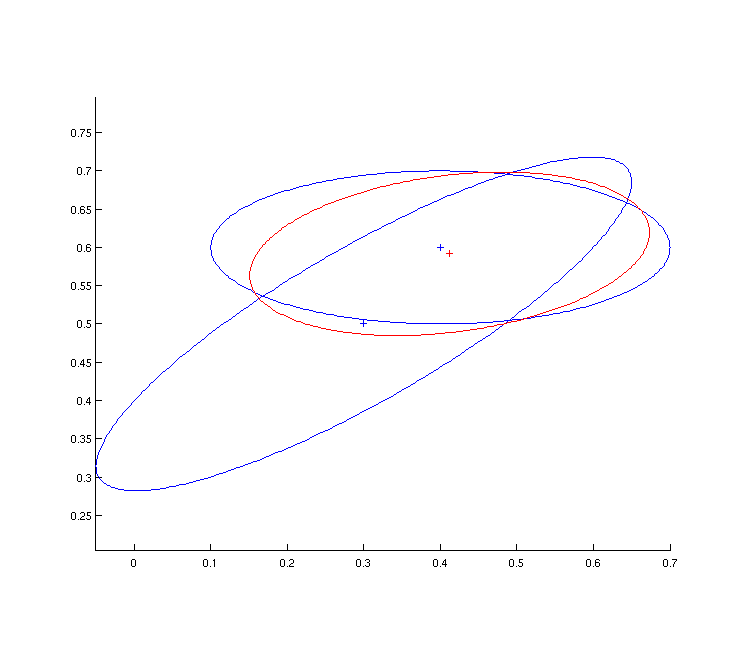
\includegraphics[width=0.4\textwidth]{figures/ci2d-25.png}}

        \subfloat[$\omega_1$=0.50]{\label{fig:ci2d50}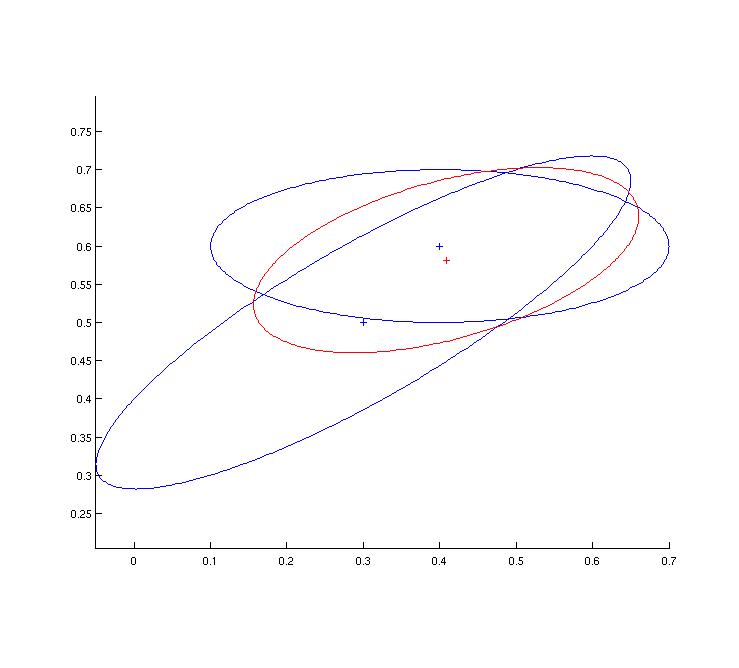
\includegraphics[width=0.4\textwidth]{figures/ci2d-50.png}}
        \subfloat[$\omega_1$=0.75]{\label{fig:ci2d75}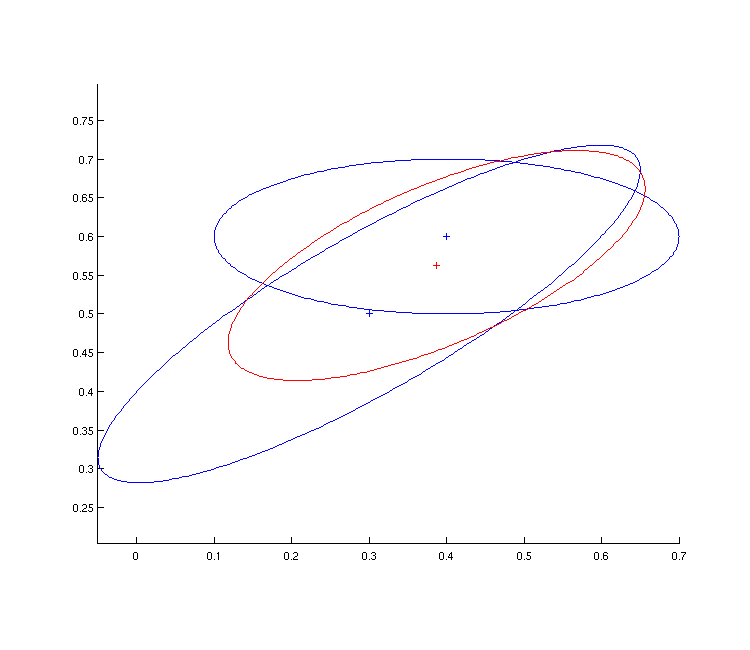
\includegraphics[width=0.4\textwidth]{figures/ci2d-75.png}}

        \subfloat[$\omega_1$=0.95]{\label{fig:ci2d95}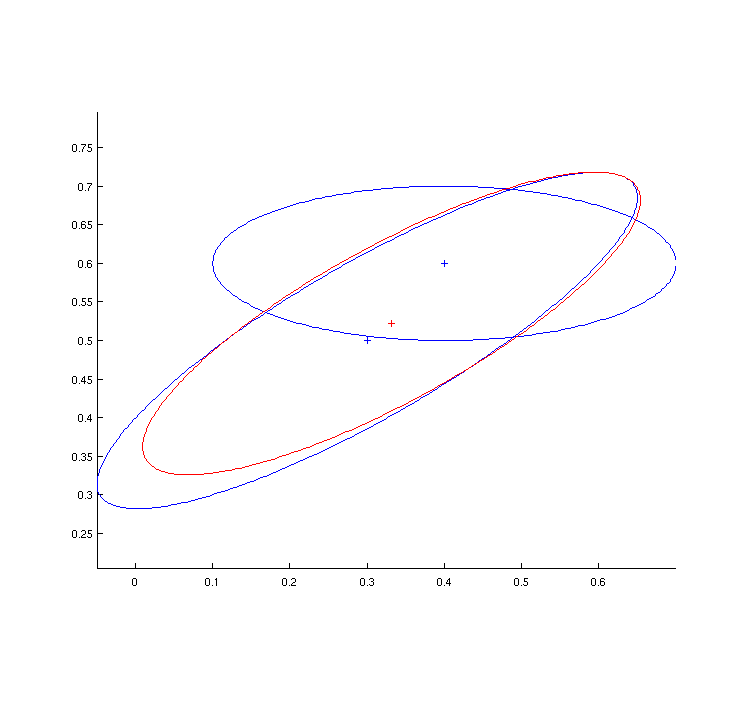
\includegraphics[width=0.4\textwidth]{figures/ci2d-95.png}}
    \caption{\it 1-$\sigma$ contour plots for two 2D input estimates (blue) together with the CI fused result (red), for
        different values of $\omega$. Note how the CI result contour behaves like an interpolation between these two
        inputs as $\omega$ varies from 0 to 1. }
    \label{fig:ci2d}
\end{figure}
\begin{align}
    \m{C} &= \left(\omega_1\m{H}_1^T\m{M}^{-1}_1\m{H}_1+\omega_2\m{H}_2^T\m{M}^{-1}_2\m{H}_2+\dots+\omega_n\m{H}_n^T\m{M}^{-1}_n\m{H}_n\right)\label{eqn:cicov}\\
    \v{c} &= \m{C}\left(\omega_1\m{H}_1^T\m{M}^{-1}_1\v{m}_1+\omega_2\m{H}_2^T\m{M}^{-1}_2\v{m}_2+\dots+\omega_n\m{H}_n^T\m{M}^{-1}_n\v{m}_n\right)\label{eqn:cimean}
\end{align}
where $\m{H}_i$ is the transformation for the state space of the fused estimate to the state space of the estimate $i$
\cite{uhlmann03,fusion01}.

Figure \ref{fig:ci2d} shows an example of CI performed on a set of two input estimates. Different CI results are shown
for different values of $\omega$ in the range $(0,1)$, and each possible result is numerically consistent. An application which
performs CI should select the appropriate $\omega$ to minimize the size, e.g. the determinant, of the fused
covariance~\cite{uhlmann03}.

To reiterate, CI requires that all of its inputs be consistent, but it will function correctly in the face of partially
or completely correlated input data \footnote{CI as described here finds the optimal fused result when the correlation
between its inputs is completely unknown; but another form of CI called Split CI is optimal when the degree of
correlation is partially known, and the estimates can be represented in split covariance form. See Appendix B
of~\cite{uhlmann03} for more information.}.



% SECTION 3 CU
\subsection{Optimal Covariance Union}\label{section:cu}

In order to develop a completely robust data fusion application, it may be necessary to handle possibly spurious
measurements prior to any data fusion being performed. If two given estimates $(\v{m}_1,\m{M}_1)$ and
$(\v{m}_2,\m{M}_2)$ are determined to be mutually inconsistent with each other, i.e. the difference between their means
is much larger than what can be expected based on their respective error covariance estimates, then using either the
Kalman filter or CI equations will yield an inconsistent fused result~\cite{uhlmann03}.

Computing the Mahalanobis distance between the two estimates,
\begin{equation}\label{eqn:mahalanobis}
(\v{m}_1-\v{m}_2)^T(\m{M}_1+\m{M}_2)^{-1}(\v{m}_1-\v{m}_2),
\end{equation}
is one method to detect statistically significant deviations between these estimates (for example, as in figure
\ref{fig:kalman2d-i}). If such a deviation is detected, it can be assumed one of the estimates is the result of
spurious measurements or corrupted data, but it may not be possible to detect which of the estimates is at
fault~\cite{uhlmann03}.

Covariance Union (CU) is a data fusion technique which can be used to resolve such a confliction by finding a union
estimate which is consistent with both (or all of) its inputs. This union $(\v{u},\m{U})$ is found by minimizing some
measure of $\m{U}$, e.g. the determinant, subject to the following constraints,
\begin{figure}[tbp]
    \centering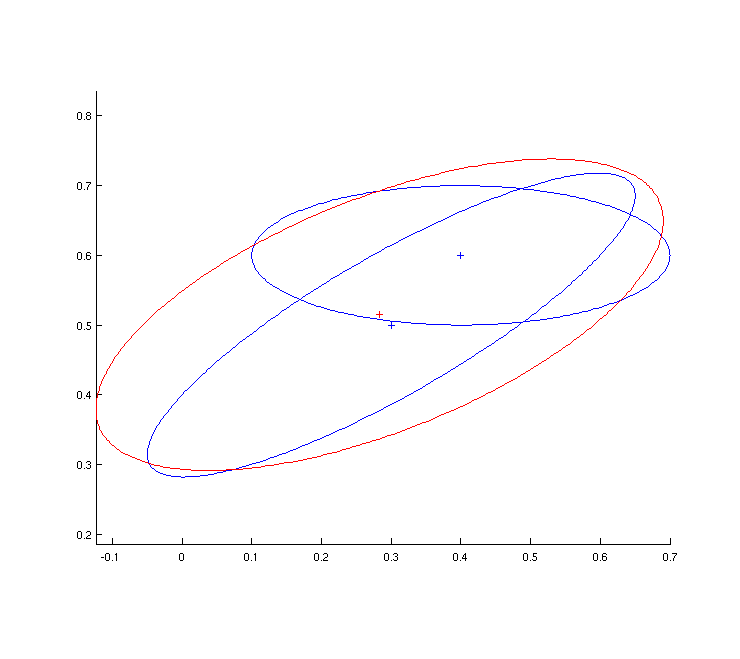
\includegraphics[width=0.6\textwidth]{figures/cu2d.png}
    \caption{\it 1-$\sigma$ contour plots of two 2D input estimates (blue) together with the CU result (red).}
    \label{fig:cu2d}
\end{figure}
\begin{align}
    \m{U}   &\geq   \m{M}_1 + (\v{u}-\v{m}_1)(\v{u}-\v{m}_1)^T\nonumber\\
    \m{U}   &\geq   \m{M}_2 + (\v{u}-\v{m}_2)(\v{u}-\v{m}_2)^T\nonumber\\
    ~       &\qquad\vdots\nonumber\\
    \m{U}   &\geq   \m{M}_n + (\v{u}-\v{m}_n)(\v{u}-\v{m}_n)^T,\label{eqn:cu}
\end{align}
for inputs $1$ to $n$. The goal of this operation is to find the location of the mean vector $\v{u}$ having the smallest
covariance $\m{U}$ that is large enough to guarantee consistency with its $n$ input estimates, regardless of which of the
$n$ estimates is consistent~\cite{fusion06,uhlmann03}.

In multimodal applications, the inputs to CU are not separate estimates of the same object to be deconflicted, but
separate modes used to represent the state of a complex or compound object. Performing CU on some or all of these modes
can be used to reduce the overall information complexity by combining modes, instead of pruning ``unimportant'' modes
(which would lead to an overestimation of the importance of the remaining modes).
This is necessary when considering the fusion of a complex set $S$ with another set $T$, which yields a combined
estimate that has $O(|S|*|T|)$ modes, formed from the Cartesian product $S\times T$. When the fused estimate exceeds the
complexity of the original estimates for each fusion step, the increasing complexity will tend to exhaust available
resources~\cite{fusion06}. The CU result is a faithful representation of all the modes it has replaced~\cite{uhlmann03}.

To reiterate, CU operates correctly even if one or more of its modes are inconsistent (as long as one is consistent), at
the cost of a much larger (less certain) error covariance that the Kalman filter or CI would provide.


% MOTIVATION for GCU
\section{Motivation for Generalized Covariance Union}\label{section:motivation}

The use of Covariance Union in data fusion is intended to guarantee consistency in the presence of spurious
data. CU is only useful if it will produce a result that is consistent with all of its inputs. However, a common
scenario arises in which CU will generate a result that is consistent with only one of its inputs (and inconsistent with
some or all of the others).

Consider the set of measurements $(\v{m}_1,\m{M}_1),(\v{m}_2,\m{M}_2),(\v{m}_3,\m{M}_3)$, which must be combined using
CU. The union may be computed in two ways:
\begin{enumerate}
\item {\em CU is applied to all three estimates simultaneously.}\\
    $(\v{u},\m{U})=\CU\left((\v{m}_1,\m{M}_1),(\v{m}_2,\m{M}_2),(\v{m}_3,\v{M}_3)\right)$
\item {\em CU is applied in a pair-wise fashion.}\\
    $(\v{u}',\m{U}')=\CU\left((\v{m}_1,\m{M}_1),(\v{m}_2,\m{M}_2)\right),$\\
    $(\v{u},\m{U})=\CU\left((\v{m}_3,\m{M}_3),(\v{u}',\m{U}')\right)$
\end{enumerate}
By its definition, given in equation \ref{eqn:cu}, the CU result is guaranteed to be consistent with its inputs. In the
first case, this means $(\v{u},\m{U})$ is consistent with $(\v{m}_1,\m{M}_1)$, $(\v{m}_2,\m{M}_2)$, and
$(\v{m}_3,\m{M}_3)$.  In the second case, however, all that is known for certain is that $(\v{u},\m{U})$ is consistent
with $(\v{m}_3,\m{M}_3)$ and $(\v{u}',\m{U}')$, and separately that $(\v{u}',\m{U}')$ is consistent with
$(\v{m}_1,\m{M}_1)$ and $(\v{m}_2,\m{M}_2)$. 
\begin{figure}[tbp]
    \centering
        \subfloat[First, the intermediate pairwise result is calculated.]{\label{fig:gcu-i1}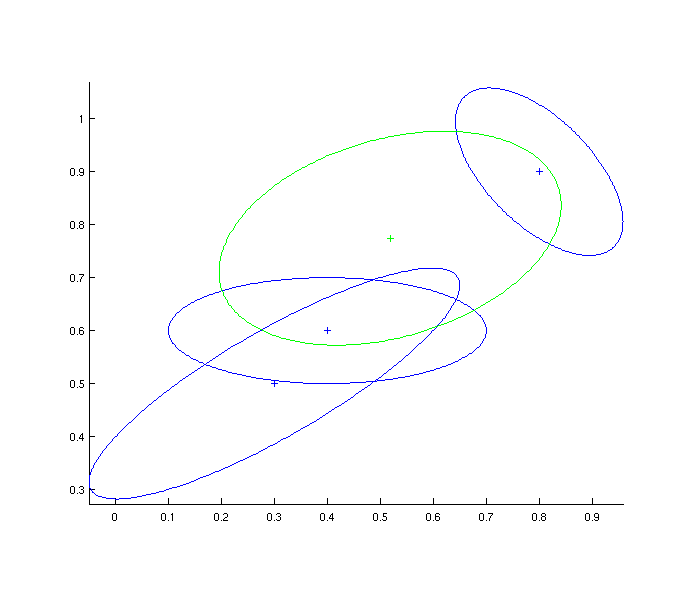
\includegraphics[width=0.4\textwidth]{figures/cu2d-i1.png}}
        \subfloat[Then, that intermediate result is used as input for the final result.]{\label{fig:gcu-iall}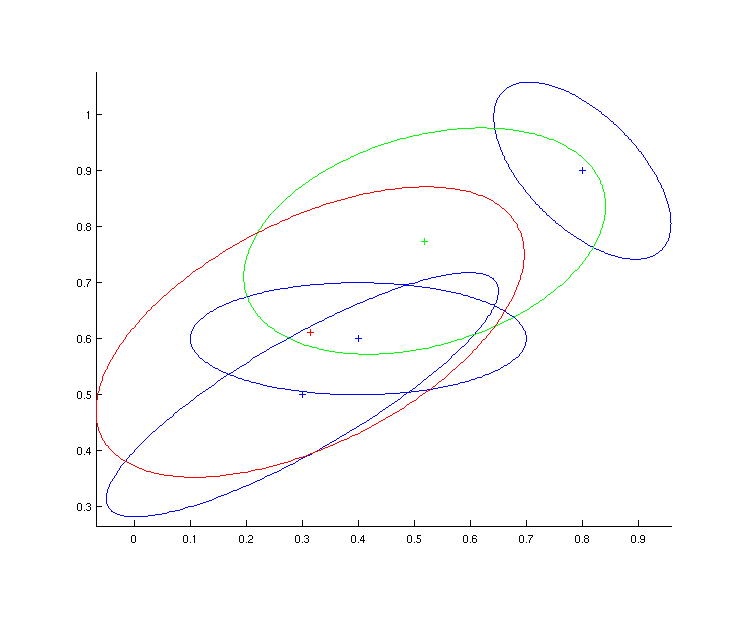
\includegraphics[width=0.4\textwidth]{figures/cu2d-iall.png}}
    \caption{\it 1-$\sigma$ contour plots of three 2D inputs (blue) together with the intermediate (pairwise) Optimal CU result
        (green) and the final (pairwise) CU result (red). Note that although the intermediate result is consistent with
        its two inputs, one of the original (blue) inputs is a clear outlier with the final (red) result.}
    \label{fig:cu2d-i}
\end{figure}

The nature of CU is to consider only the current state of the problem, i.e. its immediate inputs, and it functions with
no knowledge of any previous states. Consider an application which gathers a set of $n$ measurements at each discrete
time step, and may perform CU on some or all of those measurements for later use. If at time step $k$ CU replaces a
given estimate $(\v{m}_{i|k},\m{M}_{i|k})$ with a consistent union $(\v{u}_{k},\m{U}_{k})$, it does so by shifting the
mean from $\v{m}_{i|k}$ to $\v{u}_{k}$, and enlarging the covariance by at least the outer product of
$(\v{u}_{k}-\v{m}_{i|k})$ \cite{uhlmann03}. But if the estimate $(\v{u}_{k},\m{U}_{k})$ is used at time step $k+1$ as an
input to another CU operation, $\CU_{k+1}$ will have no knowledge of the mean shift that occurred during $\CU_{k}$. Since
CU finds the optimal, i.e. the tightest, covariance possible for all the inputs, any mean shifting that occurred during
prior time steps may cause this optimal covariance to be inconsistent for the inputs to those prior time steps
\cite{fusion06}.


% GCU
\section{Formulation of Generalized Covariance Union}\label{section:gcu}
In order to address the problems with Optimal CU as defined in section \ref{section:cu}, with regard to inconsistencies
that arise from a pair-wise or time-sequence application as described in section \ref{section:motivation}, it is
necessary to use Generalized CU. The generalized form of CU includes an additional parameter $\alpha_i$ per estimate in
the constraint equations. As with Optimal CU, the goal is to minimize some measure of $\m{U}$, e.g. the determinant. The
constraints are
\begin{figure}[tbp]
    \centering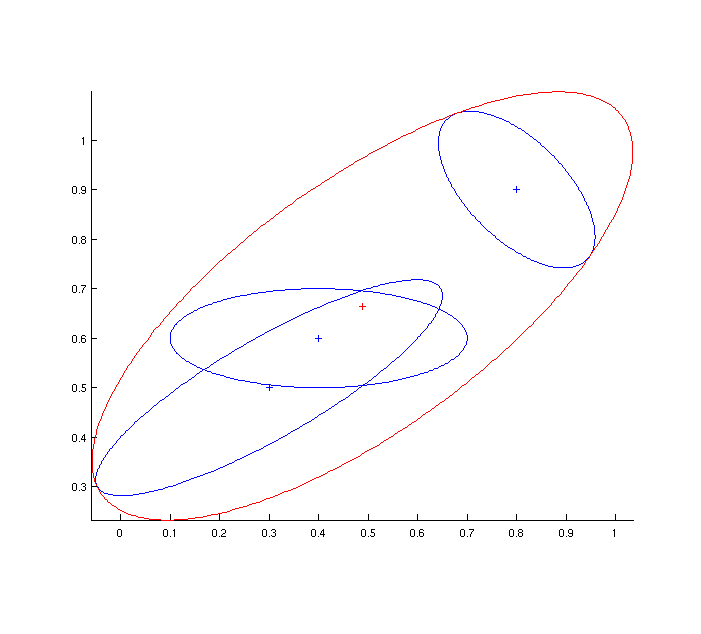
\includegraphics[width=0.6\textwidth]{figures/cu2d-gen-batch.png}
    \caption{\it 1-$\sigma$ contour plots of three 2D inputs (blue) together with the batch Generalized CU result (red).
        This is the first time that these 1-$\sigma$ plots appear to exhibit a minimally enclosing behavior.}
    \label{fig:cu2d-gen-batch}
\end{figure}
\begin{align}
    \m{U}   &\geq    \frac{\m{M}_1}{\alpha_1} + \frac{(\v{u}-\v{m}_1)(\v{u}-\v{m}_1)^T}{1-\alpha_1}\nonumber\\
    \m{U}   &\geq    \frac{\m{M}_2}{\alpha_2} + \frac{(\v{u}-\v{m}_2)(\v{u}-\v{m}_2)^T}{1-\alpha_2}\nonumber\\
    ~       &\qquad\vdots\nonumber\\
    \m{U}   &\geq    \frac{\m{M}_n}{\alpha_n} + \frac{(\v{u}-\v{m}_n)(\v{u}-\v{m}_n)^T}{1-\alpha_n},\label{eqn:gcu}
\end{align}
where $\alpha_1\dots\alpha_n$ are in the range $(0,1)$ \cite{fusion06}. Each $\alpha_i$ is equivalent to the $\omega$
parameter in equation \ref{eqn:cijointcov}~\cite{uhlmann03}, in this context used to prevent either a single covariance
$\m{M}_i$ or a single mean shift term $(\v{u}-\v{m}_i)$ from dominating the CU calculation. The $\alpha_i$ parameters
are optimized as part of this calculation to generate the tightest union possible~\cite{fusion06}. The result is
sub-optimal, but it is necessary to use this form of CU if it is used as part of a pair-wise or time-sequence
application as described above.  Generalized CU guarantees consistency regardless of how many times its result is
re-used in future CU operations.
\begin{figure}[tbp]
    \centering
        \subfloat[First, the intermediate pairwise result is calculated.]{\label{fig:gcu-s1}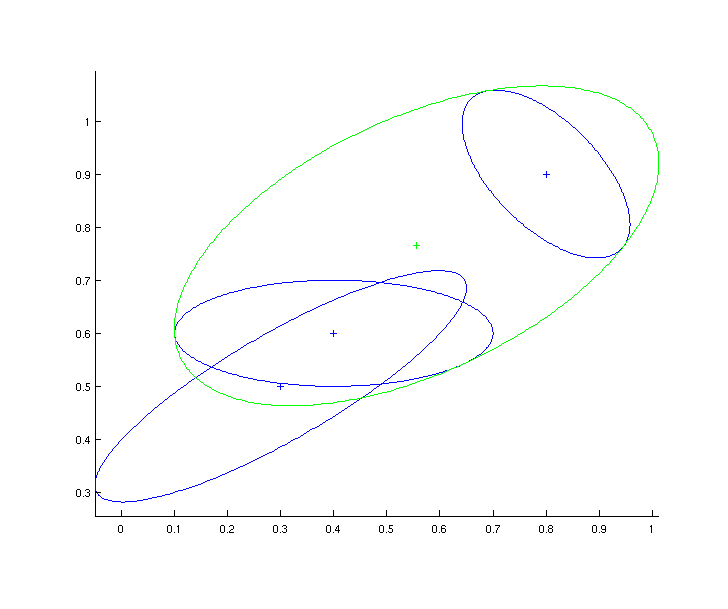
\includegraphics[width=0.4\textwidth]{figures/cu2d-gen-s1.png}}
        \subfloat[Then, that intermediate result is used as input for the final result.]{\label{fig:gcu-sall}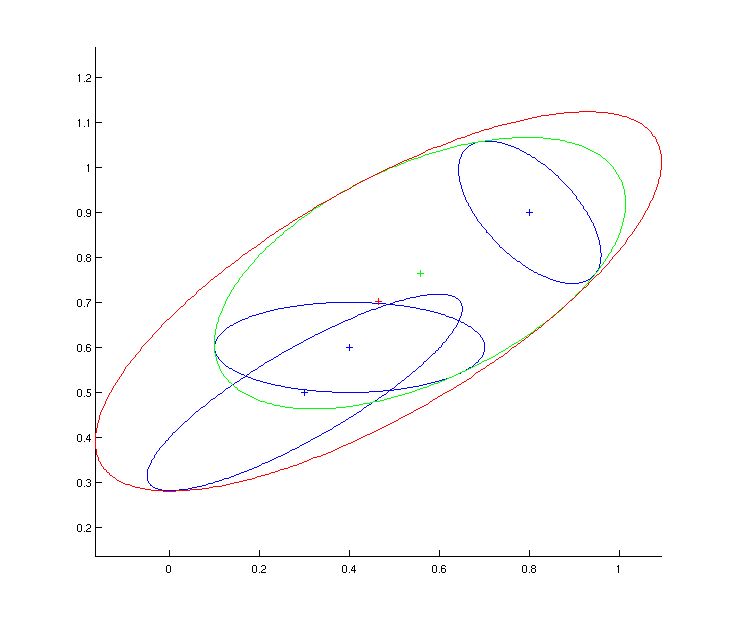
\includegraphics[width=0.4\textwidth]{figures/cu2d-gen-sall.png}}
    \caption{\it 1-$\sigma$ contour plots of three 2D inputs (blue) together with the intermediate (pairwise) Generalized CU result
        (green) and the final (pairwise) GCU result (red). Note that the final (red) result is consistent with all of
        its inputs, including all the original (blue) inputs, even those that were not used as direct inputs.}
    \label{fig:cu2d-gen-s}
\end{figure}
Figure \ref{fig:cu2d-gen-batch} shows GCU applied as a single batch operation, and figure \ref{fig:cu2d-gen-s} shows GCU
applied pairwise to the same three input estimates. The pairwise application of GCU is shown for completeness, but the
batch application is of main interest. It is this batch GCU operation, specifically its 1-$\sigma$ contour ellipsoid,
which will be compared to the MEEE problem.



